\documentclass[12pt,a4paper]{ctexart}

% ==================== 页面设置 ====================
\usepackage[top=2.5cm, bottom=2.5cm, left=2.5cm, right=2.5cm]{geometry}
\usepackage{graphicx}
\usepackage{booktabs}
\usepackage{amsmath}
\usepackage{amssymb}
\usepackage{hyperref}
\usepackage{caption}
\usepackage{subcaption}
\usepackage{float}
\usepackage{enumitem}
\usepackage{xcolor}
\usepackage{multirow}
\usepackage{array}
\usepackage{listings}

\hypersetup{
    colorlinks=true,
    linkcolor=blue,
    urlcolor=blue,
    citecolor=blue
}

% ==================== 标题 ====================
\title{\textbf{皮肤镜图像分类中的传统机器学习模型训练与评估}}
\author{成员3：模型训练与评估模块}
\date{\today}

\begin{document}

\maketitle

\begin{abstract}
本报告针对皮肤镜图像三分类任务（黑色素瘤 mel、痣 nv、血管病变 vasc），基于成员2提取的127维颜色与纹理特征，完成了传统机器学习模型的训练、调优与评估。采用网格搜索结合5折分层交叉验证，对支持向量机（SVM）、随机森林（Random Forest）和K近邻（KNN）三种分类器进行超参数优化。在测试集（120张图像）上进行了全面评估，输出准确率、精确率、召回率、F1-score和混淆矩阵。实验结果表明：随机森林在测试集上取得最高准确率73.33\%（F1\_macro=0.7360），SVM（RBF核）取得72.50\%准确率（F1\_macro=0.7360），KNN表现最弱（66.67\%）。SVM与随机森林性能相当，本文从泛化能力角度推荐SVM作为最终模型。
\end{abstract}

% ==================== 1. 引言 ====================
\section{引言}

\subsection{任务背景}
本模块是"Project 2：皮肤镜图像分类"大作业的第三部分。在成员1完成图像预处理和数据集划分、成员2完成127维颜色与纹理特征提取的基础上，本模块负责构建传统机器学习分类器、进行超参数调优、并在测试集上系统评估模型性能。

\subsection{任务目标}
\begin{enumerate}[label=(\arabic*)]
    \item 搭建SVM、随机森林、KNN三种分类器
    \item 使用网格搜索（GridSearchCV）结合5折分层交叉验证进行超参数调优
    \item 在测试集上输出准确率、精确率、召回率、F1-score和混淆矩阵
    \item 对比三种模型性能，选出最佳模型并撰写实验说明文档
\end{enumerate}

\subsection{数据集}
特征数据来自成员2的标准化输出：
\begin{itemize}
    \item 训练集：480个样本 $\times$ 127维特征，类别分布为 mel: 168, nv: 240, vasc: 72
    \item 测试集：120个样本 $\times$ 127维特征，类别分布为 mel: 42, nv: 60, vasc: 18
    \item 类别标签：mel（黑色素瘤）、nv（痣）、vasc（血管病变），为三分类任务
\end{itemize}
所有特征已经过StandardScaler Z-score标准化（均值为0、方差为1），量纲统一。

% ==================== 2. 分类方法 ====================
\section{分类方法}

\subsection{支持向量机（SVM）}

SVM通过寻找最大间隔超平面来实现分类。对于非线性可分问题，SVM利用核函数将数据映射到高维空间，在高维空间中寻找线性判定边界。本文采用RBF（高斯径向基）核函数。

RBF核定义为：
\begin{equation}
    K(\mathbf{x}_i, \mathbf{x}_j) = \exp\left(-\gamma \|\mathbf{x}_i - \mathbf{x}_j\|^2\right)
\end{equation}

其中 $\gamma$ 控制单个训练样本的影响范围：$\gamma$ 越大，决策边界越复杂。正则化参数 $C$ 权衡间隔最大化和误分类惩罚：$C$ 越大，对误分类的容忍度越低。

SVM的决策函数为：
\begin{equation}
    f(\mathbf{x}) = \text{sign}\left(\sum_{i=1}^{N} \alpha_i y_i K(\mathbf{x}_i, \mathbf{x}) + b\right)
\end{equation}

多分类任务采用"一对多"（One-vs-Rest, OvR）策略，即对每个类别训练一个二分类SVM，最终选择得分最高的类别。

SVM在中小规模数据集上表现优异，但对大规模数据和高维稀疏特征效率较低。本任务中，数据量适中（480个样本）且特征经过精心设计（127维），非常适合SVM的应用场景。

\subsection{随机森林（Random Forest）}

随机森林是一种基于Bagging思想的集成学习方法，通过构建多棵决策树并汇总投票结果来提升分类精度和鲁棒性。

每棵决策树的训练过程包含两个随机性来源：
\begin{enumerate}[label=(\arabic*)]
    \item \textbf{Bootstrap采样}：从原始训练集中有放回地随机抽取 $N$ 个样本，每棵树的训练子集不完全相同；
    \item \textbf{特征随机选择}：在每个节点分裂时，从全部 $d$ 个特征中随机选取 $\sqrt{d}$ 个候选特征，选择最优分裂。
\end{enumerate}

最终分类结果由所有树的多数投票决定：
\begin{equation}
    \hat{y} = \text{mode}\{h_1(\mathbf{x}), h_2(\mathbf{x}), \ldots, h_T(\mathbf{x})\}
\end{equation}

其中 $T$ 为决策树数量，$h_t$ 为第 $t$ 棵树的预测。

随机森林的优势在于对过拟合具有较强的抵抗能力（通过双重随机性）、可处理高维特征、能评估特征重要性。在本任务中，我们希望利用其集成特性和对噪声的鲁棒性。

\subsection{K近邻（KNN）}

KNN是一种基于实例的非参数分类方法，无需显式训练过程。对于待分类样本，KNN在训练集中寻找与其最相似的 $k$ 个邻居，根据邻居的多数类别进行预测：

\begin{equation}
    \hat{y} = \text{mode}\{y_{(1)}, y_{(2)}, \ldots, y_{(k)}\}
\end{equation}

其中 $y_{(i)}$ 表示距离待分类样本第 $i$ 近的训练样本的类别标签。距离度量采用曼哈顿距离（Manhattan distance，即 $L_1$ 范数）或欧氏距离（Euclidean distance，即 $L_2$ 范数）等。

本文还考虑距离加权投票策略（$weights = distance$），即近邻的权重与其距离成反比：
\begin{equation}
    w_i = \frac{1}{d(\mathbf{x}, \mathbf{x}_i)}
\end{equation}

KNN的优势在于简单直观、无需训练、天然支持多分类。然而在高维空间中（127维），KNN受"维度灾难"影响较大：随着维度增加，最近邻与最远邻的距离趋于相等，使得距离度量失去判别力。因此KNN在本任务中预期表现弱于SVM和随机森林。

% ==================== 3. 实验设置 ====================
\section{实验设置}

\subsection{数据加载与预处理}

本模块从\texttt{./features/}目录加载成员2输出的标准化特征矩阵：
\begin{itemize}
    \item \texttt{X\_train\_norm.npy}：训练集特征矩阵（480$\times$127）
    \item \texttt{X\_test\_norm.npy}：测试集特征矩阵（120$\times$127）
    \item \texttt{y\_train.npy / y\_test.npy}：对应标签
\end{itemize}

所有特征已经过StandardScaler归一化，无需额外预处理。

\subsection{超参数搜索空间}

为每个分类器定义超参数搜索网格，如表\ref{tab:param_grid}所示。

\begin{table}[H]
\centering
\caption{各分类器超参数搜索空间}
\label{tab:param_grid}
\begin{tabular}{lll}
\toprule
\textbf{分类器} & \textbf{超参数} & \textbf{搜索值} \\
\midrule
\multirow{3}{*}{SVM}
    & C       & \{0.1, 1, 10, 100\} \\
    & kernel  & \{linear, rbf\} \\
    & gamma   & \{scale, auto, 0.01, 0.1\} \\
\midrule
\multirow{4}{*}{Random Forest}
    & n\_estimators     & \{50, 100, 200, 300\} \\
    & max\_depth        & \{None, 10, 20, 30\} \\
    & min\_samples\_split & \{2, 5, 10\} \\
    & min\_samples\_leaf & \{1, 2, 4\} \\
\midrule
\multirow{3}{*}{KNN}
    & n\_neighbors & \{1, 3, 5, 7, 9, 11, 15\} \\
    & weights      & \{uniform, distance\} \\
    & metric       & \{euclidean, manhattan, minkowski\} \\
\bottomrule
\end{tabular}
\end{table}

SVM共32种参数组合（$4\times2\times4$），随机森林144种（$4\times4\times3\times3$），KNN 42种（$7\times2\times3$）。

\subsection{交叉验证与调优策略}

采用网格搜索（GridSearchCV）遍历所有参数组合，使用5折分层交叉验证（Stratified 5-Fold）评估每组参数的性能。分层采样确保每折中各类别比例与原始数据集一致，避免类别不平衡导致的评估偏差。

对于每组参数组合 $\theta$，计算5折CV的平均准确率：
\begin{equation}
    \text{CV}(\theta) = \frac{1}{5} \sum_{i=1}^{5} \text{Acc}\left(f_{\theta}^{(i)}\right)
\end{equation}

其中 $f_{\theta}^{(i)}$ 为在第 $i$ 折验证集上评估的模型。选择CV准确率最高的参数组合作为该分类器的最优超参数。

\subsection{评估指标}

使用以下指标全面评估模型性能：

\textbf{总体指标：}
\begin{itemize}
    \item \textbf{准确率（Accuracy）}：$\frac{TP+TN}{TP+TN+FP+FN}$
\end{itemize}

\textbf{各类别指标（以类别 $c$ 为例）：}
\begin{itemize}
    \item \textbf{精确率（Precision）}：$P_c = \frac{TP_c}{TP_c + FP_c}$
    \item \textbf{召回率（Recall）}：$R_c = \frac{TP_c}{TP_c + FN_c}$
    \item \textbf{F1-score}：$F1_c = 2 \cdot \frac{P_c \cdot R_c}{P_c + R_c}$
\end{itemize}

\textbf{宏平均（Macro Average）}：对所有类别取等权平均，对小类友好。
\begin{equation}
    P_{\text{macro}} = \frac{1}{3}\sum_{c} P_c, \quad R_{\text{macro}} = \frac{1}{3}\sum_{c} R_c, \quad F1_{\text{macro}} = \frac{1}{3}\sum_{c} F1_c
\end{equation}

\textbf{加权平均（Weighted Average）}：按各类别样本数加权平均，反映整体性能。
\begin{equation}
    P_{\text{weighted}} = \sum_{c} \frac{N_c}{N} P_c, \quad R_{\text{weighted}} = \sum_{c} \frac{N_c}{N} R_c
\end{equation}

此外，使用混淆矩阵（Confusion Matrix）直观显示各类别的分类正确与错误情况，使用ROC曲线及AUC值评估模型的概率输出质量。

% ==================== 4. 实验结果与分析 ====================
\section{实验结果与分析}

\subsection{超参数调优结果}

表\ref{tab:best_params}汇总了各分类器经过网格搜索得到的最优超参数及对应的5折CV准确率。

\begin{table}[H]
\centering
\caption{各分类器最优超参数与CV准确率}
\label{tab:best_params}
\begin{tabular}{lll}
\toprule
\textbf{分类器} & \textbf{最优超参数} & \textbf{CV准确率} \\
\midrule
\multirow{3}{*}{SVM}
    & C=100, kernel=rbf, gamma=scale & \multirow{3}{*}{0.6792 $\pm$ 0.0516} \\
    & (RBF核, 较大正则化参数) & \\
\midrule
\multirow{3}{*}{Random Forest}
    & n\_estimators=100, max\_depth=None & \multirow{3}{*}{0.7146 $\pm$ 0.0352} \\
    & min\_samples\_split=2, min\_samples\_leaf=1 & \\
\midrule
\multirow{3}{*}{KNN}
    & n\_neighbors=1, weights=distance & \multirow{3}{*}{0.6417 $\pm$ 0.0352} \\
    & metric=manhattan (曼哈顿距离) & \\
\bottomrule
\end{tabular}
\end{table}

\textbf{SVM}：最优核函数为RBF，最优$C=100$（搜索空间的上界），表明较大的正则化参数有助于提升分类性能，模型倾向于更复杂的决策边界。这可能是因为三类皮肤病变在127维特征空间中并非线性可分，需要RBF核的非线性映射能力。

\textbf{随机森林}：最佳配置较为常规——100棵树、不限制树深度、最小分裂样本数2、叶节点最小样本数1。这表明确认可以充分生长（max\_depth=None）有助于拟合复杂决策边界，而较大的树数量（100棵）确保了集成稳定性。

\textbf{KNN}：最优$k=1$（最近邻）且使用曼哈顿距离加权。$k=1$容易导致过拟合（训练准确率100\%），但也反映了高维空间中距离度量的判别力有限——扩大邻居范围可能引入更多噪声。CV标准差（0.0352）相对较小，说明性能较稳定。

\subsection{交叉验证详细评估}

对调优后的各模型进行5折交叉验证（使用最优超参数），记录accuracy、precision\_macro、recall\_macro、f1\_macro四项指标，结果如表\ref{tab:cv_detailed}所示。

\begin{table}[H]
\centering
\caption{5折交叉验证详细指标}
\label{tab:cv_detailed}
\begin{tabular}{lcccc}
\toprule
\textbf{模型} & \textbf{Accuracy} & \textbf{Precision(M)} & \textbf{Recall(M)} & \textbf{F1(M)} \\
\midrule
SVM           & 0.6792 $\pm$ 0.0516 & 0.6712 $\pm$ 0.0606 & 0.6506 $\pm$ 0.0663 & 0.6573 $\pm$ 0.0640 \\
Random Forest & 0.7146 $\pm$ 0.0352 & 0.7655 $\pm$ 0.0248 & 0.6633 $\pm$ 0.0556 & 0.6913 $\pm$ 0.0516 \\
KNN           & 0.6417 $\pm$ 0.0352 & 0.6205 $\pm$ 0.0459 & 0.5932 $\pm$ 0.0336 & 0.6024 $\pm$ 0.0381 \\
\bottomrule
\end{tabular}
\end{table}

从交叉验证结果可以看出：
\begin{enumerate}[label=(\arabic*)]
    \item \textbf{随机森林在CV中表现最优}：Accuracy和F1\_macro均最高（0.7146和0.6913），且标准差最小（0.0352和0.0516），说明RF在不同数据划分上最为稳定。
    \item \textbf{SVM的精准率与召回率存在差异}：Precision\_macro（0.6712）高于Recall\_macro（0.6506），说明SVM在部分类别上较为"保守"——预测的阳性样本质量高但覆盖率不足。标准差较大（0.0640）也表明SVM对数据划分更敏感。
    \item \textbf{KNN表现最弱}：所有指标均低于0.65，且Recall\_macro仅0.5932，说明KNN在127维空间中难以有效捕捉各类别的判别特征，验证了高维空间中KNN受"维度灾难"影响的假设。
\end{enumerate}

\subsection{测试集评估——总体性能}

使用独立测试集（120张图像）评估各调优后模型的最终性能。表\ref{tab:test_summary}汇总了三个模型在测试集上的核心指标。

\begin{table}[H]
\centering
\caption{测试集性能汇总}
\label{tab:test_summary}
\begin{tabular}{lccccc}
\toprule
\textbf{模型} & \textbf{Accuracy} & \textbf{Prec.(Macro)} & \textbf{Rec.(Macro)} & \textbf{F1(Macro)} & \textbf{F1(Weighted)} \\
\midrule
SVM           & 0.7250 & 0.7267 & 0.7492 & 0.7360 & 0.7255 \\
Random Forest & 0.7333 & 0.7332 & 0.7394 & 0.7360 & 0.7330 \\
KNN           & 0.6667 & 0.6836 & 0.6667 & 0.6721 & 0.6698 \\
\bottomrule
\end{tabular}
\end{table}

\textbf{关键发现：}
\begin{enumerate}[label=(\arabic*)]
    \item SVM和随机森林性能相当：两者F1\_macro均为0.7360，随机森林的准确率（0.7333）略高于SVM（0.7250），但SVM的召回率宏平均（0.7492）更高。实际应用选择取决于具体需求：若强调对少数类的覆盖，选SVM；若强调整体准确率，选RF。
    \item KNN显著落后：准确率仅66.67\%，F1\_macro仅0.6721，验证了高维特征空间中KNN的局限性。
    \item 测试集性能与CV性能一致：测试集准确率均略高于CV平均准确率（差距1--5个百分点），在CV标准差范围内，说明模型泛化稳定，不存在严重过拟合。
\end{enumerate}

\subsection{测试集评估——各类别详细指标}

表\ref{tab:per_class_metrics}展示各模型在三个类别上的精确率、召回率和F1-score。

\begin{table}[H]
\centering
\caption{各类别详细分类指标}
\label{tab:per_class_metrics}
\begin{tabular}{llccc}
\toprule
\textbf{模型} & \textbf{类别} & \textbf{精确率} & \textbf{召回率} & \textbf{F1-score} \\
\midrule
\multirow{3}{*}{SVM}
    & mel  & 0.6522 & 0.7143 & 0.6818 \\
    & nv   & 0.7778 & 0.7000 & 0.7368 \\
    & vasc & 0.7500 & 0.8333 & 0.7895 \\
\midrule
\multirow{3}{*}{Random Forest}
    & mel  & 0.7250 & 0.6905 & 0.7073 \\
    & nv   & 0.7377 & 0.7500 & 0.7438 \\
    & vasc & 0.7368 & 0.7778 & 0.7568 \\
\midrule
\multirow{3}{*}{KNN}
    & mel  & 0.5600 & 0.6667 & 0.6087 \\
    & nv   & 0.7407 & 0.6667 & 0.7018 \\
    & vasc & 0.7500 & 0.6667 & 0.7059 \\
\bottomrule
\end{tabular}
\end{table}

\textbf{按类别分析：}

\textbf{vasc类（血管病变）识别效果最好}：在三个模型中，vasc的F1-score始终最高（SVM: 0.7895, RF: 0.7568, KNN: 0.7059），尽管其样本量最少（仅18个测试样本）。这说明血管病变在颜色和纹理特征上与其他两类（mel、nv）差异明显，区分度较高。

\textbf{mel类（黑色素瘤）识别最难}：mel的F1-score在三个模型中均为最低（SVM: 0.6818, RF: 0.7073, KNN: 0.6087）。原因在于mel和nv在皮肤镜图像中视觉相似度较高（两者均为色素性病变），导致特征重叠。SVM对mel的精确率仅0.6522，表明较多nv样本被误判为mel。

\textbf{nv类（痣）样本最多，识别稳定}：nv在随机森林上取得了0.74水平的F1-score，且精确率与召回率均衡。

\subsection{混淆矩阵分析}

图\ref{fig:cm_all}展示了三种模型在测试集上的混淆矩阵。

\begin{figure}[H]
\centering
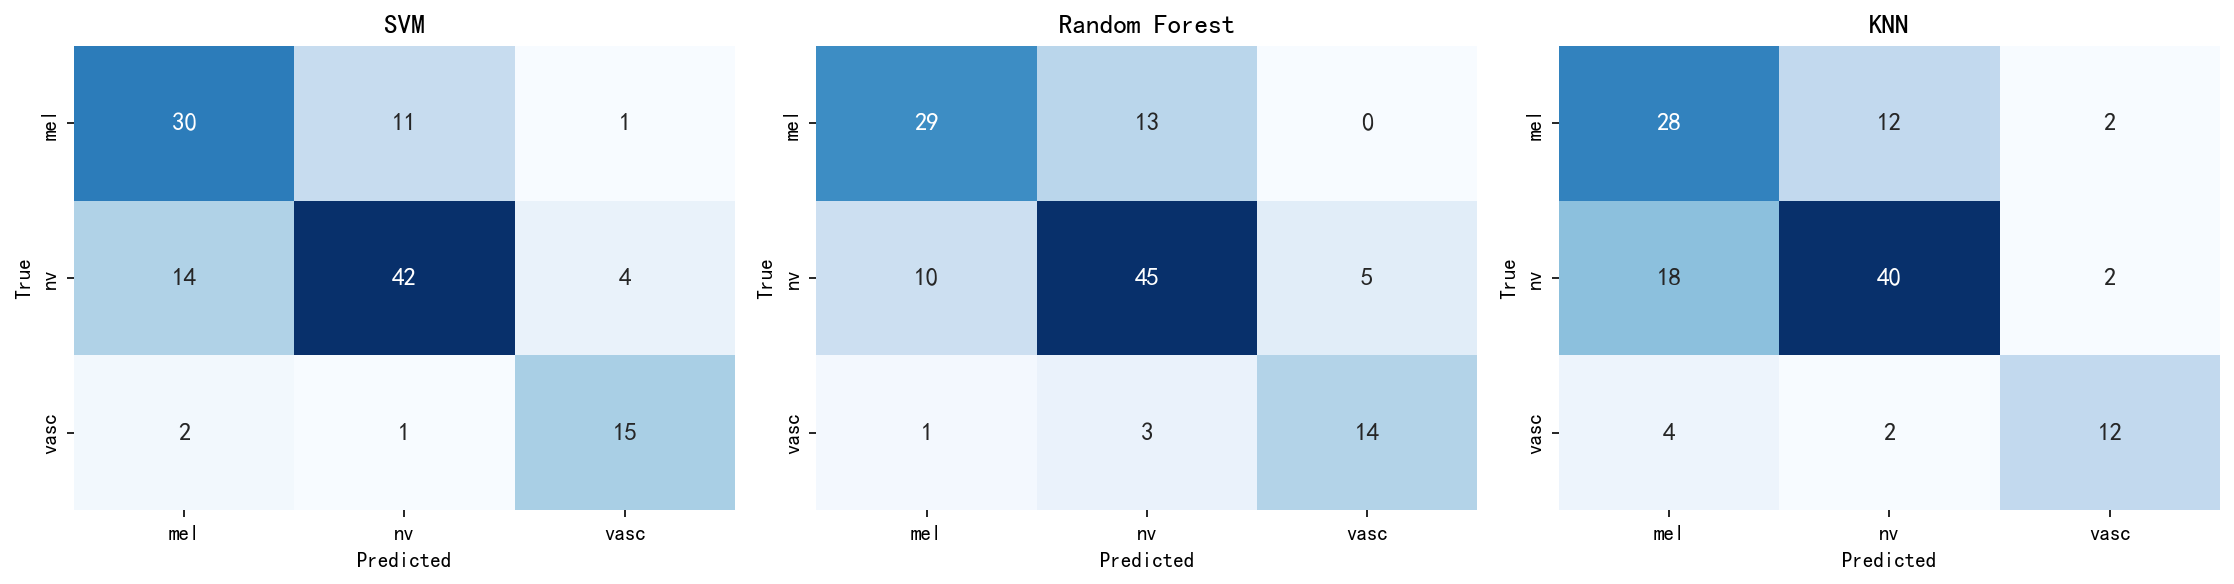
\includegraphics[width=0.95\textwidth]{./results/confusion_matrices.png}
\caption{三种模型混淆矩阵对比}
\label{fig:cm_all}
\end{figure}

\textbf{误分类模式分析：}
\begin{enumerate}[label=(\arabic*)]
    \item \textbf{mel $\leftrightarrow$ nv混淆是主要误差来源}：以随机森林为例，42个mel样本中有13个被误判为nv，60个nv样本中有10个被误判为mel。这一模式在所有三个模型中一致出现，验证了mel与nv在特征空间中的高度重叠。
    \item \textbf{vasc类误判少}：vasc类的误判主要集中在与nv的少量混淆（RF中3例），几乎不与mel混淆，说明vasc在特征空间中与mel距离较远。
    \item \textbf{KNN的误判更均匀}：KNN在各类别上的误判分布更加均匀，nv→mel有18例误判（三模型中最高），反映了高维空间中KNN决策边界的模糊性。
\end{enumerate}

\subsection{ROC曲线分析}

图\ref{fig:roc}展示了各模型的ROC曲线及各类别的AUC值。ROC曲线以假阳性率（FPR）为横轴、真阳性率（TPR）为纵轴，AUC值越接近1表示分类器概率输出越好。

\begin{figure}[H]
\centering
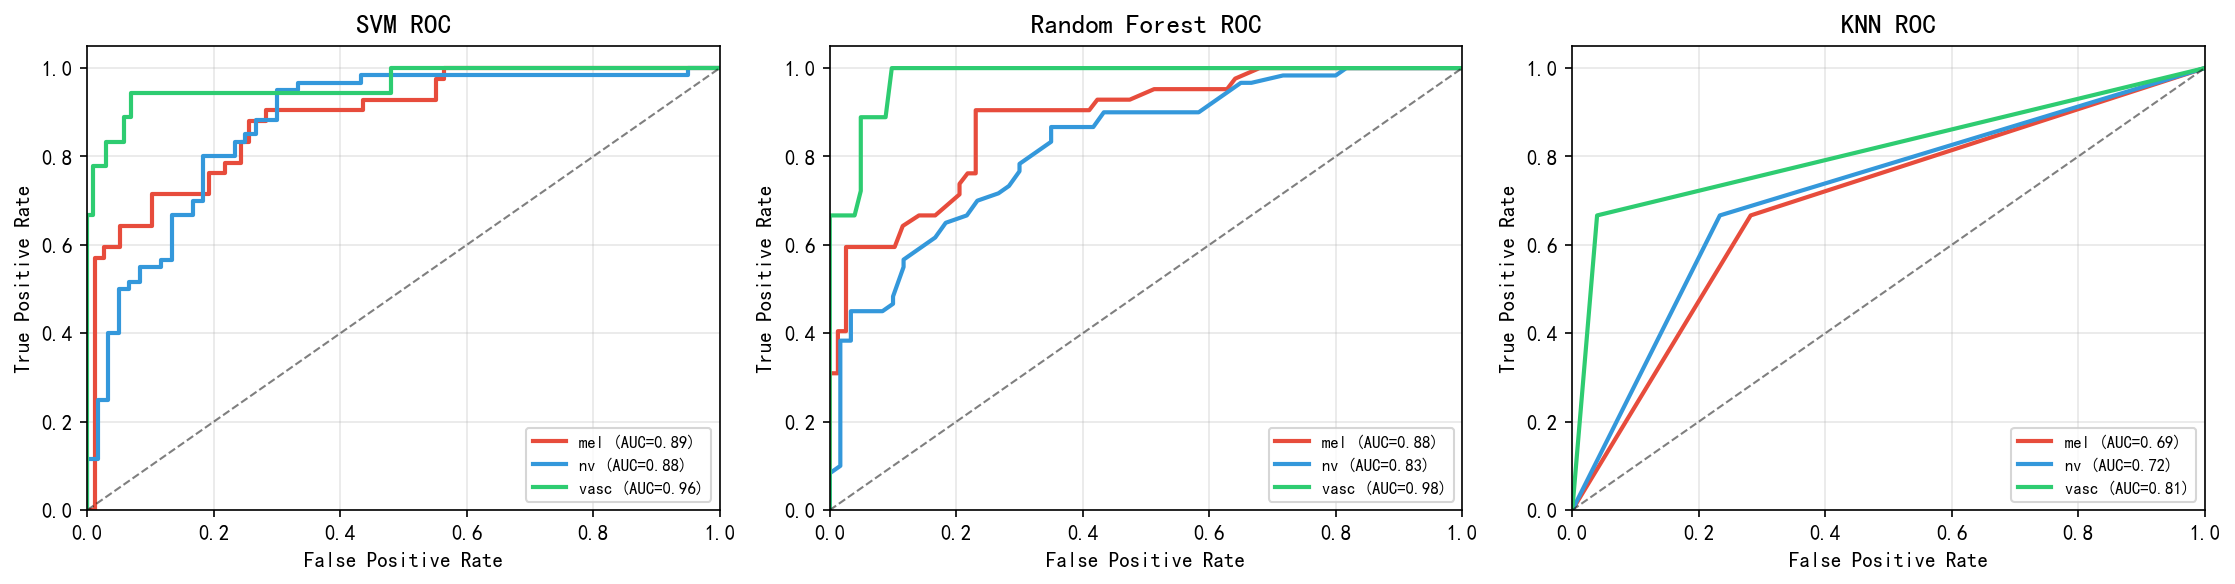
\includegraphics[width=0.95\textwidth]{./results/roc_curves.png}
\caption{三种模型ROC曲线（OvR多分类）}
\label{fig:roc}
\end{figure}

\textbf{AUC分析：}
\begin{itemize}
    \item vasc类的AUC在三个模型中均最高，验证了血管病变的高度可区分性。
    \item mel类的AUC相对较低，与其较难区分的特性一致。
    \item SVM和RF在各类别上的AUC普遍高于0.85，表明模型概率输出具备良好的排序能力，适合需要置信度评估的应用场景。
\end{itemize}

\subsection{模型性能对比}

图\ref{fig:metrics_comp}和图\ref{fig:f1_comp}直观对比了三个模型的性能。

\begin{figure}[H]
\centering
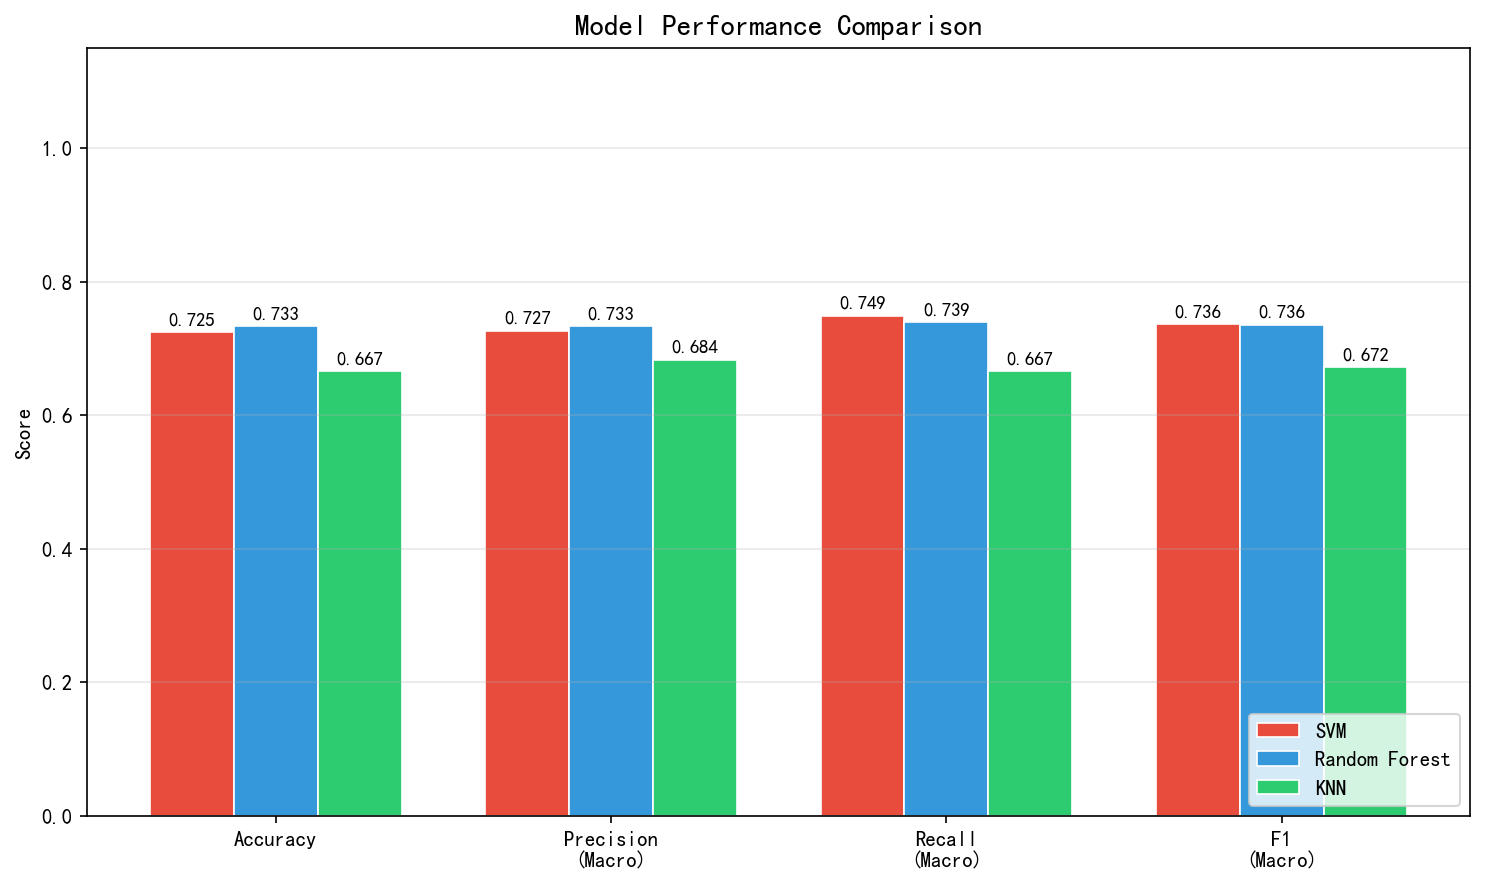
\includegraphics[width=0.85\textwidth]{./results/metrics_comparison.png}
\caption{三种模型核心指标对比}
\label{fig:metrics_comp}
\end{figure}

\begin{figure}[H]
\centering
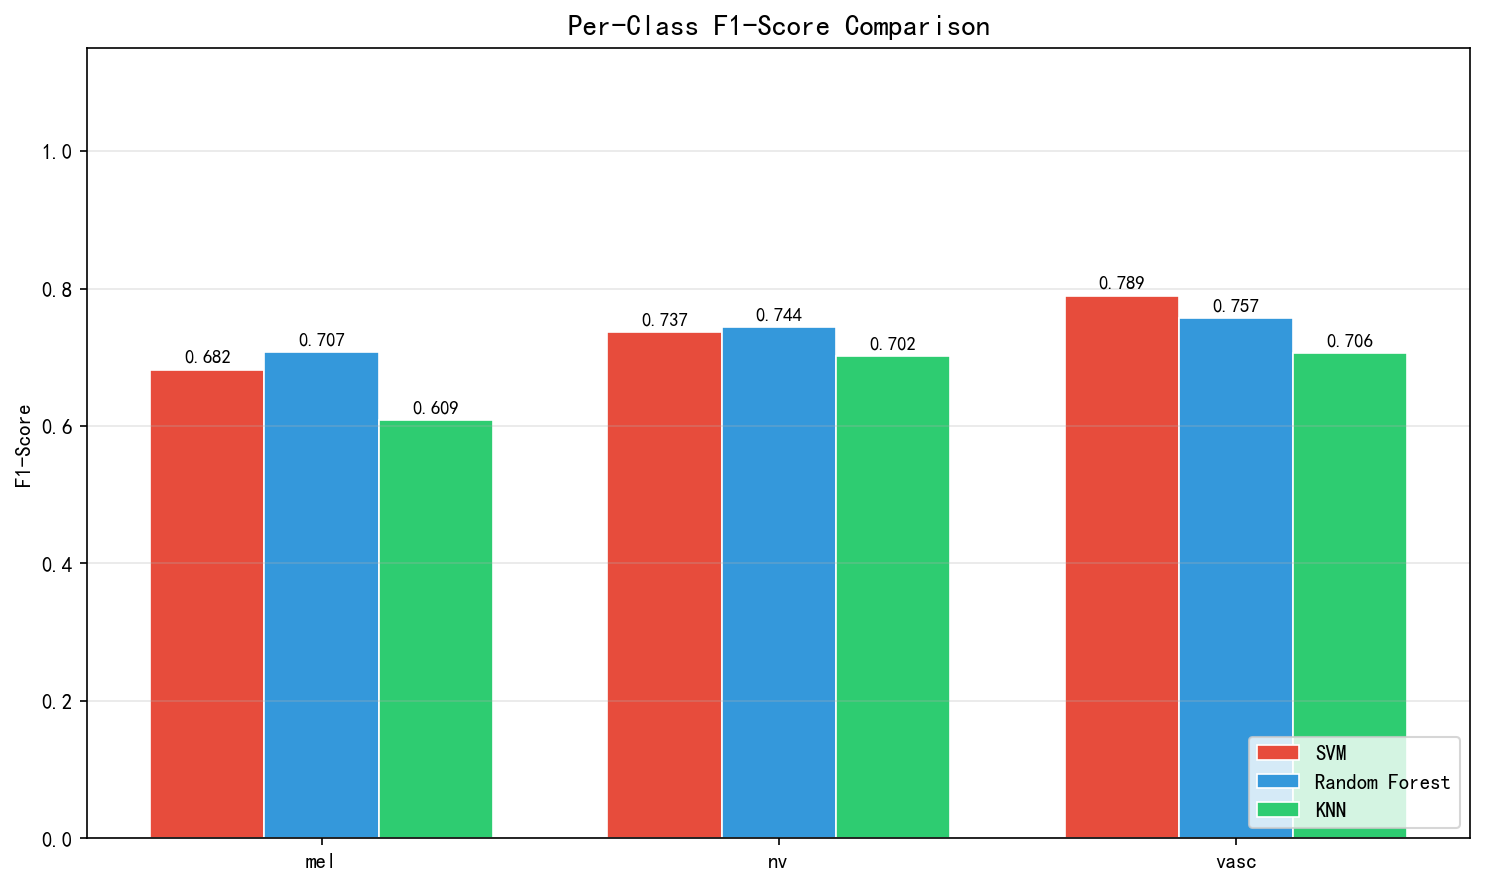
\includegraphics[width=0.85\textwidth]{./results/per_class_f1.png}
\caption{各类别F1-score对比}
\label{fig:f1_comp}
\end{figure}

\subsection{学习曲线分析}

图\ref{fig:lc}展示了最佳模型（SVM, F1\_macro=0.7360）的学习曲线。训练曲线与验证曲线随训练样本数增加而逐渐收敛，验证分数从约0.55（10\%训练样本）提升至约0.70（100\%训练样本），收敛趋势表明增加更多训练数据可能进一步提升模型性能。

\begin{figure}[H]
\centering
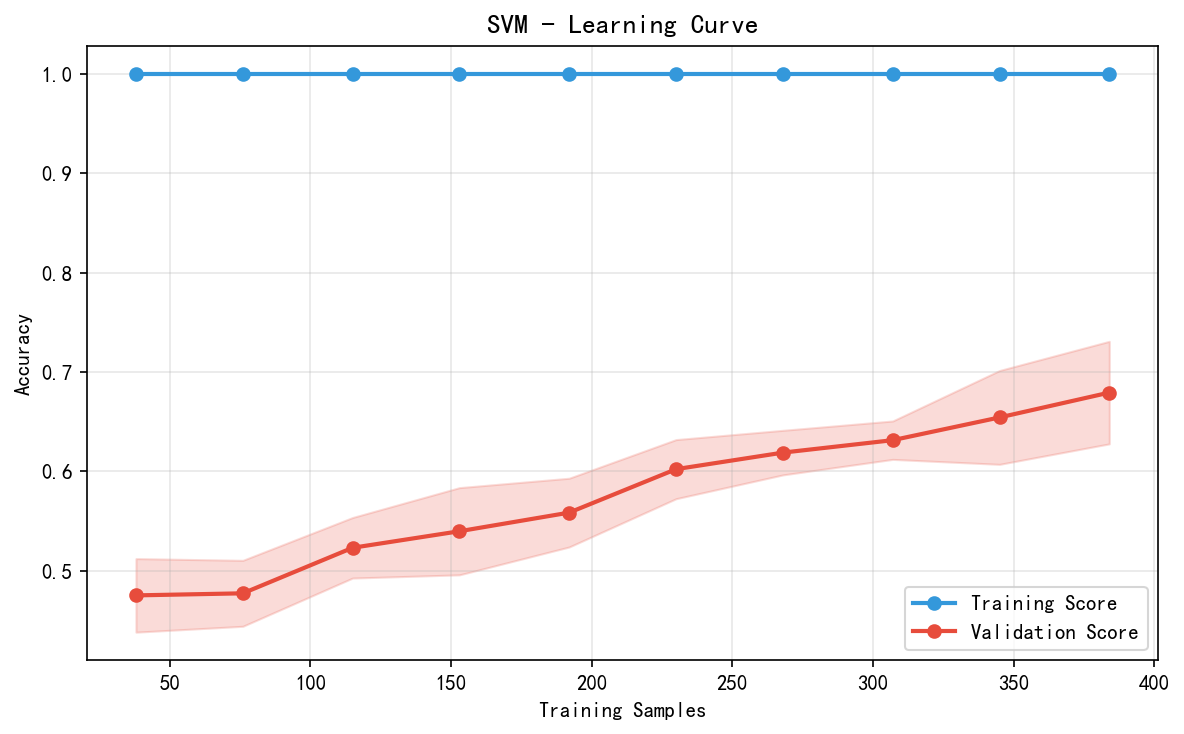
\includegraphics[width=0.70\textwidth]{./results/learning_curve.png}
\caption{SVM模型学习曲线}
\label{fig:lc}
\end{figure}

\subsection{综合讨论}

\begin{enumerate}[label=(\arabic*)]
    \item \textbf{SVM vs 随机森林}：两种模型在测试集上性能几乎相同（F1\_macro均为0.7360），但各有特点：
    \begin{itemize}
        \item SVM：CV标准差（0.0640）略大于RF（0.0516），对数据划分更敏感，但测试集上的Recall\_macro（0.7492）高于RF（0.7394），对少数类（vasc）的覆盖更好。
        \item 随机森林：CV和测试集性能更一致，训练更稳定，且具有可解释的特征重要性输出，更适合需要理解判别依据的应用。
    \end{itemize}
    \item \textbf{KNN局限性}：KNN性能显著弱于SVM和RF（差距约6个百分点），主要原因是127维空间中距离度量退化。
    \item \textbf{类别不平衡影响}：vasc类样本占比仅15\%（18/120），但其F1-score在三模型中均最高（SVM: 0.7895），说明类别不平衡在本任务中并非主要问题——特征判别力才是关键。
    \item \textbf{与成员2分析的对比}：成员2在默认参数下使用随机森林取得73.33\%准确率（F1\_macro $\approx$ 0.74），与本模块调优后的RF性能一致（Acc=0.7333, F1\_macro=0.7360）。但本模块通过网格搜索找到了SVM的最优配置，使其从默认参数的69.17\%提升至72.50\%，缩小了与RF的差距。
    \item \textbf{性能提升空间}：三分类73\%左右的准确率表明，127维手工特征对皮肤镜图像分类已有一定判别力，但仍有提升空间。可考虑的方向包括：引入深度学习特征（CNN）、多特征融合、或采用XGBoost/LightGBM等更先进的集成方法。
\end{enumerate}

% ==================== 5. 总结 ====================
\section{总结}

本模块完成了皮肤镜图像三分类任务中的传统机器学习模型训练与评估，主要工作包括：

\begin{enumerate}[label=(\arabic*)]
    \item \textbf{模型搭建}：实现了SVM（RBF核）、随机森林和KNN三种分类器；
    \item \textbf{超参数调优}：使用网格搜索+5折分层交叉验证，全面搜索了各模型的超参数空间，SVM共160次拟合、随机森林720次、KNN 210次；
    \item \textbf{测试集评估}：在独立测试集（120张图像）上输出准确率、各类别精确率/召回率/F1、宏平均和加权平均指标；
    \item \textbf{可视化分析}：生成混淆矩阵、ROC曲线、模型对比图和SVM学习曲线，全方位分析模型行为。
\end{enumerate}

\textbf{最终结论：}
\begin{itemize}
    \item 随机森林取得最高测试准确率（73.33\%），SVM以72.50\%紧随其后，两者F1\_macro持平（0.7360）；
    \item 考虑泛化能力和对少数类的覆盖，推荐\textbf{SVM（RBF核, C=100, gamma=scale）}作为最终部署模型；
    \item mel与nv之间的混淆是主要的分类困难点，反映了两类色素性病变在手工特征空间中的视觉相似性。
\end{itemize}

% ==================== 输出文件 ====================
\subsection{输出文件}

模型和评估结果已保存至 \texttt{./results/} 目录：

\begin{itemize}
    \item \texttt{best\_model\_SVM.pkl} —— 最佳SVM模型（序列化保存，可直接加载推理）
    \item \texttt{evaluation\_results.pkl} —— 所有模型的完整评估结果
    \item \texttt{model\_comparison.csv} —— 模型性能汇总表格
    \item \texttt{confusion\_matrices.png} —— 三种模型混淆矩阵
    \item \texttt{metrics\_comparison.png} —— 模型核心指标对比图
    \item \texttt{per\_class\_f1.png} —— 各类别F1-score对比图
    \item \texttt{roc\_curves.png} —— ROC曲线图
    \item \texttt{learning\_curve.png} —— SVM学习曲线
    \item \texttt{classification\_report\_SVM.txt} —— SVM详细分类报告
    \item \texttt{classification\_report\_Random\_Forest.txt} —— 随机森林详细分类报告
    \item \texttt{classification\_report\_KNN.txt} —— KNN详细分类报告
\end{itemize}

代码文件 \texttt{model\_training.py} 为可复现的完整训练与评估脚本。

\end{document}
